%!TEX root = bug-taxo.tex

\section{Study Design}

The goal of this study is to analyze the location of bug fixes, with the purpose of classifying bug fixes into types.
More specifically, this study aims to answer the folliwing two research questions:

\begin{itemize}
	\item {\bf RQ$_1$:} {\it What are the proportions of different types of bugs?} This research question aims to what extent bug can be classified according to their fix-locations and the proportion of each types.
  Specifically, we investigate if different types of bugs exists at all and if the proportion of different types in non-negligible.
  As discussed ealier, knowing, for example, that bugs of Type 2 and 4 are the most predominant ones suggests that we need to investigate techniques to help detect whether an incoming bug is of Types 2 and 4 by examining historical data.
  Similarly, if we can automatically identify a bug that is related to another one that has been fixed then we can reuse the results of reproducing the first bug in reproducing the second one.

	\item {\bf RQ$_2$:} {\it How complex is each type of bugs?} This second research question aims to investigate the complexity of the different types of bug.
  More specifically, we analyze and discuss the complexity of different types of bugs using code and process metrics both.
  For the code aspect of the complexity, we compute the number of different files impacted by the fix and the number of hunks and churns.
  We do not compute any statical complexity metrics such as cyclomatic complexity \cite{McCabe1989}.
  For the process aspect of complexity, we analyze the severity of the bug, the amount of duplicate bug report submitted, the number of times a bug report gets reopened, the number of comments and the time required to fix the bug.

\end{itemize}

\subsection{Context Selection}

The context of this study consists of the change history of 388 projects belonging to two software ecosystem, namely, Apache and Netbeans.
Tbale \ref{table:datasets} reports, for each of them, (i) the number of projects analyzed, (ii) size ranges in terms of the number of classes and KLOC, (iii) the overall number of commits and issues analyzed, and (iv) the average, minimum, and maximum length of the projects' story (in years).

\begin{table}[h]
\begin{center}
\begin{tabular}{@{}c|c|c|c|c@{}}
\textbf{Dataset} & \textbf{R/F BR} & \textbf{CS} & \textbf{Files} & \textbf{Projects} \\ \hline \hline
Netbeans         & 53,258          & 122,632     & 30,595         & 39                \\
Apache           & 49,449          & 106,366     & 38,111         & 349               \\
Total            & 102,707         & 229,153     & 68,809         & 388               \\ \hline \hline

\end{tabular}
\end{center}

\caption{Datasets\label{table:datasets}}
\end{table}



All the analysed projects are hosted in {\it Git} or {\it Mercurial} repositories and have either a {\it Jira} or a {\it Bugzilla} issue tracker associated with it.
The Apache ecosystem consists in 349 projects written in various programming languages (C, C++, Java, Python, ...) and uses {\it Git} and {\it Jira}.
These projects represent the Apache ecosystem in its entirety; no system has been excluded from our study.
The complete list can be found online\footnote{https://projects.apache.org/projects.html?name}.
The Netbeans ecosystem consists in 39 projects mostly written in Java.
Similarly to the Apache ecosystem, we did not select some of the projects belonging to the Netbeans ecosystem but all of them.
The Netbeans community uses {\it Bugzilla} and {\it Mercurial}.

The choice of the ecosystems to analyze is not random, but rather driven by the motivation to consider projects having (i) different sizes, (ii) different architectures, and (iii) different development bases and processes.
Indeed, Apache project are extremely various in terms of size of the development team, purpose and technical choices \cite{Bavota2013}.
On the other side, Netbeans have a relatively stable list of core developer and a common vision shared through the 39 related projects \cite{Wang2011}.

Cumulatively, these datasets span from 2001 to 2014. In summary, our consolidated dataset contains 102,707 bugs, 229,153 changesets, 68,809 files that have been modified to fix the bugs, 462,848 comments, and 388 distinct systems.
We also collected 221 million lines of code modified to fix the bugs, identified 3,284 sub-projects, and 17,984 unique contributors to these bug report and source code version management systems.
The cumulated opening time for all the bugs reaches 10,661 working years (3,891,618 working days) which translates into more than one billion dollars\cite{Usnews}.

\subsection{Data Extraction and Analysis}

This subsection describes the data extraction and analysis process that we followed to answer our research questions.

\subsubsection{What are the proportions of different types of bugs?} To answer {\bf RQ$_1$}, we cloned the 349 {\it git} repositories belonging to the Apache ecosystem and the 39 {\it mercurial} repositories belonging to the Netbeans ecosystem.
The raw size of the cloned source code alone, exluding binaries, images and other non-text file, is 163 GB.
Then, we extracted all the 102,707 closed issue that have been resolved using the {\it RESOLVED/FIXED} tags.
Indeed, this study aims to classify bugs according to their fix locations.
If an issue is fixed by other means than {\it fixing} the source code, then, it falls outside the scope our study.
In order to assign commits to issues we used is the regular expression-based approach by Fischer et al. \cite{Fischer} matching the issue ID in the commit note.
Using this technic, we were able to link almost 40\% (40,493 out of 102,707) of our resolved/fixed issues to 229,153 commits.
An issue can be fixed with several commits.

We choose not to use more complex technics like ReLink, an approach proposed by Wu et al.\cite{Wu2011}, which considers the following constraints: (i) matching the committer/authors with issue tracking contributor name/email; (ii) the time interval between the commit and the last comment posted by the same author/contributor on the issue tracker must be less than seven days; and (iii) Vector Space Model (VSM) cosine similarity between the commit note and the last comment referred above or greater than 0.7 because we belive that mining more than forty thousands issues is enough to be significant.

Using our generated consolidated dataset, we extracted the files $f_i$ impacted by each commit $c_i$ for each one of our 388 projects.
Then, we classify the bugs according to the following:

\begin{itemize}
  \item {\bf Type 1:} A bug is tagged type 1 if it is fixed by modifying a file $f_i$ and $f_i$ is not involved in any other bug fix.
  \item {\bf Type 2:} A bug is tagged type 2 if it is fixed by modifying several files $f_{i..n}$ and the files $f_{i..n}$ are not involved in any other bug fix.
  \item {\bf Type 3:} A bug is tagged type 3 if it is fixed by modifying a file $f_{i}$ and the file $f_{i}$ is involved in fixing other bugs.
  \item {\bf Type 4:} A bug is tagged type 4 if it is fixed by modifying several files $f_{i..n}$ and the files $f_{i..n}$ are involved in any other bug fix.
\end{itemize}

To answer this question, we analyze whether any type is predominant in the studied ecosystem, by testing the null hypothesis:

\begin{itemize}
	\item $H_{01A}$ : The proportion of Types does not
change significantly across the studied ecosystems
\end{itemize}

We test this hypothesis by observing both a ``global'' (across ecosystem) and a ``local'' predominance (per ecosystem) of the different types of bugs.
We must observe these two aspects to ensure that the predominance of a particular type of bug is not circumstantial (in few given systems only) but is also not due to some other, unknown factors (in all systems but not in a particular ecosystem).

We answer {\bf RQ$_1$} in two steps.
The first step is to use descriptive statistics; we compute the ratio of each types to the total number of bugs in the dataset.

In the second step, we compare the proportions of the different types of bugs with respect to the ecosystem where the bugs were found.
We build the contingency table with these two qualitative variables (the type and studied ecosystem) and test the null hypothesis {\bf H$_{01A}$} to assess whether the proportion of a particular type of bugs is related to a specific ecosystem or not.

We use the Pearson's chi-squared test to reject the null hypothesis $H_{01A}$.
Pearson's chi-squared independence test is used to analyze the relationship between two qualitative data, in our study the type bugs and the studied ecosystem.
The results of Pearson's chi-squared independence test are considered
statistically significant at $\alpha$ = 0.05.
If p-value $\le$ 0.05, we reject the null hypothesis $H_{01A}$ and conclude that the proportion of each types is different for each ecosystem.

Overall, the data extraction and manipulation for {\bf RQ$_1$} (i.e., cloning repositories, linking commits to issues and tagging issues by type) took thirteen weeks on two Linux servers having 1 quadcore
3.10 GHz CPU and 12 Gb of RAM each.

\subsubsection{How complex is each type of bugs?}  To answer {\bf RQ$_2$} we went through our 40,493 of our resolved/fixed issues and the linked 229,153 commits in order to compute code and process metrics for each of them.
These metrics will then be used to assess the complexity of a bug.
The computed process metrics are:

\begin{itemize}
  \item The time $t$ it took to resolve issue $i$.
  \item The number of issues $dup$ tagged as duplicate of issue $i$.
  \item The number of time issue $i$ got reopen $reop$.
  \item The number of comments $comment$ on issue $i$.
  \item The severity $sev$ of the issue $i$.
\end{itemize}

The computed code metrics are:

\begin{itemize}
  \item The number of files $f$ impacted by issue $i$.
  \item The number of commit $c$ required to fix the issue $i$.
  \item The number of hunks $h$ required to fix the issue $i$.
  \item The number of churns $ch$ required to fix the issue $i$.
\end{itemize}


We address the relation between types and the complexity of the bugs in using our metrics.
We analyze whether Types 2 and 4 bugs are more complex to handle than Types 1 and 3 bugs, by testing the null hypotheses:

\begin{itemize}
 \item  $H_{02S}$ : The severity of different types is not significantly different
 \item  $H_{02D}$ : Different types are not significantly more likely to get duplicated.
 \item  $H_{02R}$ : Different types are not significantly more likely to get reopened.
 \item $H_{02T}$ : There is no statistically-significant difference
between the duration of fixing of different types.
\end{itemize}

For each hypothesis, we build a contingency table with the qualitative variables type of bugs and the dependent variable.

We use the Pearson's chi-squared test to reject the null
hypothesis $H_{02D}$ (respectively $H_{02R}$ ) and $H_{02S}$. The results of Pearson's chi-squared independence test are considered
statistically significant at $\alpha$ = 0.05.
If a p-value $\le$ 0.05, we reject the null hypothesis $H_{02D}$ (respectively $H_{02R}$) andconclude the fact that the bug is more likely to be duplicated (respectively reopened) is related to the type of the bug and we reject $H_{02S}$ and conclude that the severity level of the bug is related to the bug type.

\section{Analysis of the Results}



This section reports the analysis of the results achieved
aiming at answering our two research questions.

\subsection{What are the proportions of different types of bugs?}

% Please add the following required packages to your document preamble:
% \usepackage{multirow}
\begin{table*}[]
\centering
\small
\caption{Contingency table and Pearson's chi-squared tests}
\label{tab:contingency-table}
\begin{tabular}{cccccc}
Ecosystem & T1                 & T2               & T3                & T4                & Pearson's chi-squared p-Value                          \\ \rowcolor{gray!25}
Apache    & 1968  (14.3 \%)   & 1248  (9.1 \%)  & 3101  (22.6 \%)  &7422  ( 54 \%)    &  \\ \rowcolor{gray!25}
Netbeans  & 776  (2.9 \%)     & 240  (0.9 \%)   & 8372  (31.3 \%)  & 17366  (64.9 \%) &  \textless0.01                               \\ \rowcolor{gray!25}
Overall   & 2744  (6.8 \%)    & 1488  (3.7 \%)  & 11473  (28.3 \%) & 24788  (61.2 \%) &                                \\
          & \multicolumn{2}{c}{Types 1 and 2}     & \multicolumn{2}{c}{Types 3 and 4}     &                           \\ \rowcolor{gray!25}
Apache    & \multicolumn{2}{c}{3216  (23.4 \%)}  & \multicolumn{2}{c}{10523  (76.6 \%)} & \\ \rowcolor{gray!25}
Netbeans  & \multicolumn{2}{c}{1016  (3.8 \%)}   & \multicolumn{2}{c}{25738  (96.2 \%)} & \textless0.01                               \\ \rowcolor{gray!25}
All       & \multicolumn{2}{c}{4232  (10.5 \%)}  & \multicolumn{2}{c}{36261  (89.5 \%)} &                                \\
          & \multicolumn{2}{c}{Types 1 and 3}     & \multicolumn{2}{c}{Types 2 and 4}     &                           \\ \rowcolor{gray!25}
Apache    & \multicolumn{2}{c}{5069  (36.9 \%)}  & \multicolumn{2}{c}{8670  (63.1 \%)}  &  \\ \rowcolor{gray!25}
Netbeans  & \multicolumn{2}{c}{9148  (34.2 \%)}  & \multicolumn{2}{c}{17606  (65.8 \%)} &   \textless0.01                             \\ \rowcolor{gray!25}
All       & \multicolumn{2}{c}{14217  (35.1 \%)} & \multicolumn{2}{c}{26276  (64.9 \%)} &
\end{tabular}
\end{table*}


Table \ref{tab:contingency-table} presents a contingency table and the results of the Pearson's chi-squared tests we performed on each types of bug.
In addition to presenting bug types 1 to 4,  Table \ref{tab:contingency-table} also presents regroupement of bug types:
(a) Types 1 and 2 versus Types 3 and 4 and (b) Types 1 and 3 versus Types 2 and 4.


Types 3 (22.6\% and 54\%) and 4 (31.3\% and 64.9\%) are predominants compared to types 1 (14.3\% and 9.1\%) and 2 (6.8\% and 3.7\%) for the Apache and the Netbeans ecosystems, respectively.
Obviously, this observation also holds for when the two ecosystems are combined.
Overall, the proportion of different types of bug is as follows: 6.8\%, 3.7\%, 28.3\%, 61.2\% for types 1, 2, 3 and 4, respectively.
The result of the Pearson's tests are bellow 0.01.
As a reminder, we consider results of Pearson's tests statistically significant at $\alpha \textless0.05$.
Consequently, we can conclude that there is a predominance of Types 3 and 4 in all different ecosystems and this observation is not related to a specific ecosystem.
When combined into our first group, Types 1 \& 2 versus. Types 3 \& 4, there are significantly more Types 3 and 4 (89.5 \%) than Types 1 and 2 (10.5 \%).
In the second group, Types 1 \& 3 versus. Types 2 \& 4, there are significantly more Types 2 \& and 4 (64.9\%) than Types 1 \& 3 (35.1\%).



\subsection{How complex is each type of bugs?}

To answer {\bf RQ$_2$}, we analyse the complexity of each bug in terms of duplication, fixing time, comments, reopenning, files impacted, severity, changesets, hunks and chunks.

Figure \ref{fig:boxplots} presents nine boxplots describing our complexity metric for each types of each ecosystem.
In each sub-figure, the boxplots are organised as follows: (a) Types 1 to 4 of the Apache ecosystem, (b) Types 1 to 4 of the Netbeans ecosystem and (c) Types 1 to 4 of both ecosystems combined.
For all the metrics, except the severity, the median is close to zero and we can observe many outliers.
Tables \ref{tab:apache-eco}, \ref{tab:netbeans-eco} and \ref{tab:overall-eco} present descriptive statistics about each metric for each type for the Apache ecosystem, the Netbeans ecosystem and both ecosystems combined, respectively.
The descriptive Statistics used are $\mu$:mean, $\sum$:sum, $\hat{x}$:median, $\sigma$:standard deviation and $\%$:percentage.
In addition, to the descriptive statistics, these tables present matrixes of Mann-Whitney test for each metric and type.
We added the \checkmark~symbol to the Mann-Whitney test results columns when the value is statistically significant (e.g. $\alpha \textless 0.05$) and \xmark~otherwise.
Tables \ref{tab:combined-one} and \ref{tab:combined-two} are built similarly to Tables \ref{tab:apache-eco}, \ref{tab:netbeans-eco} and \ref{tab:overall-eco} at the exception that they present the data of types groups: Types 1 \& 2 vs. Types 3 \& 4 and Types 1 \& 3 vs. Types 2 \& 4.
Finally, Table \ref{tab:chi-rq2} presents the Pearson's chi-squared tests results for each complexity metrics for Types 1 to 4 and our two types combination.
In what follows, we present our findings for each complexity metric.
omplexity metrics are divided in two groups: (a) process and (b) code metrics.
Process metrics refer to metrics that have been extracted from the project tracking system (i.e. fixing time, comments, reopening and severity).
Code metrics are directly computed using the source code used to fix a given bug (i.e. files impacted, changesets required, hunks and chunks).
We acknowledge that these complexity metrics only represent an abstraction of the actual complexity of a given bug as they cannot account for the actual thought processes and expertise required to craft a fix.
However, we believe that they are an accurate abstraction.
Moreover, they are used in several studies in the field also rely on these metrics to accurately approximate the complexity of bug \cite{Weiß2007,Saha2014,Nam2013,Anvik2006,Nagappan}.

\begin{figure*}
\centering
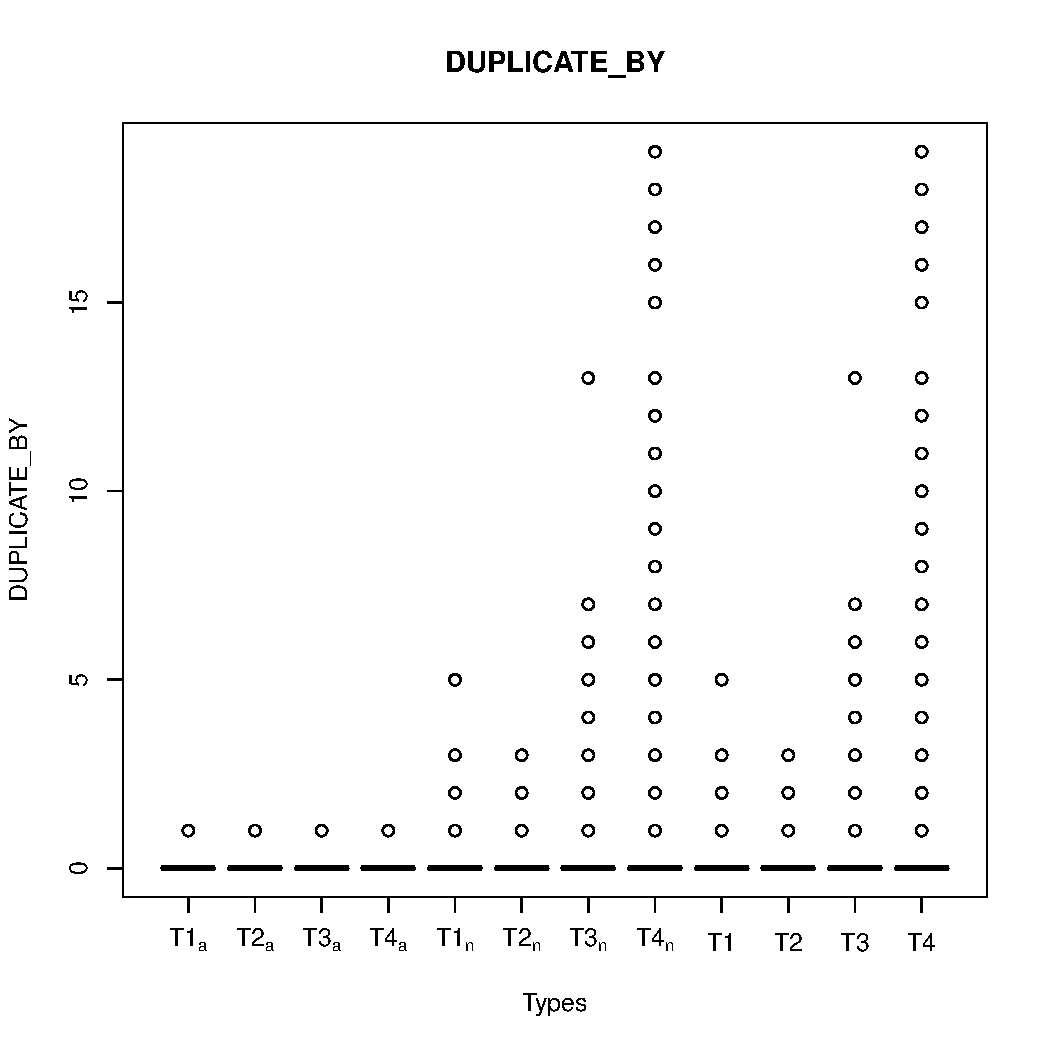
\includegraphics[page=1, width=0.30\textwidth]{extract/Rplots}
\includegraphics[page=2, width=0.30\textwidth]{extract/Rplots}
\includegraphics[page=3, width=0.30\textwidth]{extract/Rplots} \\
\includegraphics[page=4, width=0.30\textwidth]{extract/Rplots}
\includegraphics[page=5, width=0.30\textwidth]{extract/Rplots}
\includegraphics[page=6, width=0.30\textwidth]{extract/Rplots} \\
\includegraphics[page=7, width=0.30\textwidth]{extract/Rplots}
\includegraphics[page=8, width=0.30\textwidth]{extract/Rplots}
\includegraphics[page=9, width=0.30\textwidth]{extract/Rplots}

\caption{Complexity metrics boxplots. From left to right and top to bottom: Duplicate, Fixing time, Comments, Reopening, Files impacted, Severity, Changesets, Hunks and Chunks.
\label{fig:boxplots}}

\end{figure*}


\subsubsection{Duplicate}
The duplicate metric represents the number of time a bug gets resolved using the {\it duplicate} label while referencing one of the {\it resolved/fixed} bug of our dataset.
The process metric is useful to approximate the impact of a given bug on the community.
Indeed, for a bug to be resolved using the {\it duplicate}, it means that the bug has been reported before.
The more a bug gets reported by the community, the more people are impacted enough to report it.
Note that, for a bug$_a$ to be resolved using the {\it duplicate} label and referencing bug$_b$, bug$_b$ does not have to resolved itself.
Indeed, bug$_b$ could be under investigation (i.e. {\it unconfirmed}) or being fixed (i.e. {\it new} or {\it assigned}).

In the Apache ecosystem, the types that are the most likely to get duplicated, ordered by ascending mean duplication rate, are T3 (0.016) $\textless$ T2 (0.022) $\textless$ T1 (0.026) $\textless$ T4 (0.029) and they represent 14.8\%, 8.1\%, 14.5\% and 62.6\% of the total duplications, respectively.
The differences between duplication means by types, however, are only significant in 33.33\% (4/12) of the case.
Indeed, the mean duplication are only significant on the following cases: T1 vs. T3, T3 vs. T4.
For the Apache ecosystem, we can conclude that $T4_{dup}^1 \gg T1_{dup}^2 \gg T3_{dup}^4$.
We use the notation  $x_{m}^r \gg y_{m}^r$ ($x_{m}^r \ll y_{m}^r$) to represent that $x$, along the metric $m$, is significantly greater (lower) than $y$, along the same metric, according to the mann-whitney tests ($\alpha \textless 0.05$).
$r$ represents the rank of $x$ ($y$) according to $m$ from 1 (higher percentage) to 4 (lower percentage).





Netbeans T1 0.086 (2.5\%) T2 0.067 (0.6\%) T3 0.074 (23.3\%) T4 0.113 (73.6\%)

Overall T1 0.043 (3.9\%) T2 0.03 (1.5\%) T3 0.058 (22.3\%) T4 0.088 (72.3\%)

\subsubsection{Fixing time}
\subsubsection{Comments}
\subsubsection{Reopening}
\subsubsection{Severity}
\subsubsection{Files impacted}
\subsubsection{Changesets}
\subsubsection{Hunks}
\subsubsection{Chunks}




%!TEX root = ..bug-taxo.tex

% Please add the following required packages to your document preamble:
% \usepackage{graphicx}
\begin{table*}[]
\centering
\samll
\setlength\extrarowheight{6pt}
\caption{My caption}
\label{my-label}
\begin{tabular}{ccccccc|ccccc}

Types & Metric &$^\mu$ & $^\sum$ & $^\hat{x}$ & $^\sigma$ & $^\%$ & T1 & T2 & T3 & T4 \\ \hline \rowcolor{gray!25}
& Dup. & 0.026 & 51 & 0 & 0.2 & 14.8 & n.a & \xmark (0.53) & \checkmark  (\textless 0.05) & \xmark (0.45)  \\ \rowcolor{gray!25}
& Tim. & 91.574 & 180217 & 4 & 262 & 21.8 & n.a & \checkmark  (\textless 0.05) & \checkmark  (\textless 0.05) & \checkmark  (\textless 0.05)  \\ \rowcolor{gray!25}
& Com. & 4.355 & 8571 & 3 & 4.7 & 9.5 & n.a & \checkmark  (\textless 0.05) & \xmark (0.17) & \checkmark  (\textless 0.05)  \\ \rowcolor{gray!25}
& Reo. & 0.062 & 122 & 0 & 0.3 & 13.8 & n.a & \xmark (0.29) & \checkmark  (\textless 0.05) & \checkmark  (\textless 0.05)  \\ \rowcolor{gray!25}
T1 & Fil. & 0.991 & 1950 & 1 & 0.1 & 3.7 & n.a & \checkmark  (\textless 0.05) & \xmark (0.28) & \checkmark  (\textless 0.05)  \\ \rowcolor{gray!25}
& Sev. & 3.423 & 6737 & 4 & 1.3 & 13.2 & n.a & \xmark (0.18) & \checkmark  (\textless 0.05) & \checkmark  (\textless 0.05)  \\ \rowcolor{gray!25}
& Cha. & 1 & 1968 & 1 & 0 & 1.9 & n.a & \checkmark  (\textless 0.05) & \checkmark  (\textless 0.05) & \checkmark  (\textless 0.05)  \\ \rowcolor{gray!25}
& Hun. & 3.814 & 7506 & 3 & 2.4 & 0 & n.a & \checkmark  (\textless 0.05) & \checkmark  (\textless 0.05) & \checkmark  (\textless 0.05)  \\ \rowcolor{gray!25}
& Chur. & 18.761 & 36921 & 7 & 48.6 & 0 & n.a & \checkmark  (\textless 0.05) & \xmark (0.09) & \checkmark  (\textless 0.05)  \\


 & Dup. & 0.022 & 28 & 0 & 0.1 & 8.1 & \xmark (0.53) & n.a & \xmark (0.16) & \xmark (0.19)  \\
 & Tim. & 115.158 & 143717 & 8 & 294.1 & 17.4 & \checkmark  (\textless 0.05) & n.a & \checkmark  (\textless 0.05) & \checkmark  (\textless 0.05)  \\
 & Com. & 5.041 & 6291 & 4 & 4.7 & 7 & \checkmark  (\textless 0.05) & n.a & \checkmark  (\textless 0.05) & \checkmark  (\textless 0.05)  \\
 & Reo. & 0.071 & 89 & 0 & 0.3 & 10.1 & \xmark (0.29) & n.a & \checkmark  (\textless 0.05) & \xmark (0.59)  \\
T2 & Fil. & 4.381 & 5468 & 2 & 20.4 & 10.5 & \checkmark  (\textless 0.05) & n.a & \checkmark  (\textless 0.05) & \checkmark  (\textless 0.05)  \\
 & Sev. & 3.498 & 4365 & 4 & 1.2 & 8.6 & \xmark (0.18) & n.a & \checkmark  (\textless 0.05) & \checkmark  (\textless 0.05)  \\
 & Cha. & 4.681 & 5842 & 2 & 20.4 & 5.5 & \checkmark  (\textless 0.05) & n.a & \checkmark  (\textless 0.05) & \checkmark  (\textless 0.05)  \\
 & Hun. & 561.995 & 701370 & 14 & 13628.2 & 3.9 & \checkmark  (\textless 0.05) & n.a & \checkmark  (\textless 0.05) & \checkmark  (\textless 0.05)  \\
 & Chur. & 14184.869 & 17702716 & 88 & 400710.2 & 8 & \checkmark  (\textless 0.05) & n.a & \checkmark  (\textless 0.05) & \checkmark  (\textless 0.05)  \\

 \rowcolor{gray!25}
 & Dup. & 0.016 & 50 & 0 & 0.1 & 14.5 & \checkmark  (\textless 0.05) & \xmark (0.16) & n.a & \checkmark  (\textless 0.05)  \\ \rowcolor{gray!25}
 & Tim. & 35.892 & 111300 & 1 & 151.8 & 13.5 & \checkmark  (\textless 0.05) & \checkmark  (\textless 0.05) & n.a & \checkmark  (\textless 0.05)  \\ \rowcolor{gray!25}
 & Com. & 4.422 & 13712 & 3 & 4.4 & 15.2 & \xmark (0.17) & \checkmark  (\textless 0.05) & n.a & \checkmark  (\textless 0.05)  \\ \rowcolor{gray!25}
 & Reo. & 0.033 & 101 & 0 & 0.2 & 11.5 & \checkmark  (\textless 0.05) & \checkmark  (\textless 0.05) & n.a & \checkmark  (\textless 0.05)  \\ \rowcolor{gray!25}
 T3 & Fil. & 0.994 & 3081 & 1 & 0.1 & 5.9 & \xmark (0.28) & \checkmark  (\textless 0.05) & n.a & \checkmark  (\textless 0.05)  \\ \rowcolor{gray!25}
 & Sev. & 3.644 & 11300 & 4 & 1.1 & 22.2 & \checkmark  (\textless 0.05) & \checkmark  (\textless 0.05) & n.a & \checkmark  (\textless 0.05)  \\ \rowcolor{gray!25}
 & Cha. & 1 & 3101 & 1 & 0 & 2.9 & \checkmark  (\textless 0.05) & \checkmark  (\textless 0.05) & n.a & \checkmark  (\textless 0.05)  \\ \rowcolor{gray!25}
 & Hun. & 4.022 & 12472 & 3 & 3.4 & 0.1 & \checkmark  (\textless 0.05) & \checkmark  (\textless 0.05) & n.a & \checkmark  (\textless 0.05)  \\ \rowcolor{gray!25}
 & Chur. & 16.954 & 52573 & 6 & 49.8 & 0 & \xmark (0.09) & \checkmark  (\textless 0.05) & n.a & \checkmark  (\textless 0.05)  \\


& Dup. & 0.029 & 216 & 0 & 0.2 & 62.6 & \xmark (0.45) & \xmark (0.19) & \checkmark  (\textless 0.05) & n.a  \\
& Tim. & 52.76 & 391586 & 4 & 182.2 & 47.4 & \checkmark  (\textless 0.05) & \checkmark  (\textless 0.05) & \checkmark  (\textless 0.05) & n.a  \\
& Com. & 8.313 & 61701 & 5 & 10.2 & 68.3 & \checkmark  (\textless 0.05) & \checkmark  (\textless 0.05) & \checkmark  (\textless 0.05) & n.a  \\
& Reo. & 0.077 & 570 & 0 & 0.3 & 64.6 & \checkmark  (\textless 0.05) & \xmark (0.59) & \checkmark  (\textless 0.05) & n.a  \\
T4 & Fil. & 5.633 & 41805 & 3 & 14 & 79.9 & \checkmark  (\textless 0.05) & \checkmark  (\textless 0.05) & \checkmark  (\textless 0.05) & n.a  \\
& Sev. & 3.835 & 28466 & 4 & 1 & 56 & \checkmark  (\textless 0.05) & \checkmark  (\textless 0.05) & \checkmark  (\textless 0.05) & n.a  \\
& Cha. & 12.861 & 95455 & 4 & 52.2 & 89.7 & \checkmark  (\textless 0.05) & \checkmark  (\textless 0.05) & \checkmark  (\textless 0.05) & n.a  \\
& Hun. & 2305.868 & 17114149 & 30 & 58094.7 & 96 & \checkmark  (\textless 0.05) & \checkmark  (\textless 0.05) & \checkmark  (\textless 0.05) & n.a  \\
& Chur. & 27249.773 & 202247816 & 204 & 320023.5 & 91.9 & \checkmark  (\textless 0.05) & \checkmark  (\textless 0.05) & \checkmark  (\textless 0.05) & n.a

\end{tabular}%
\end{table*}

%!TEX root = ..bug-taxo.tex

\begin{table*}[]
\centering
\small
\setlength\extrarowheight{6pt}
\caption{My caption}
\label{my-label}
\begin{tabular}{ccccccc|ccccc}

Types & Metric &$^\mu$ & $^\sum$ & $^\hat{x}$ & $^\sigma$ & $^\%$ & T1 & T2 & T3 & T4 \\ \hline \rowcolor{gray!25}

& Dup. & 0.086 & 67 & 0 & 0.4 & 2.5 & n.a & \xmark (0.39) & \xmark (0.24) & \xmark (0.86) \\  \rowcolor{gray!25}
& Tim. & 92.759 & 71981 & 10 & 219.1 & 2.3 & n.a & \checkmark  (\textless 0.05) & \xmark (0.15) & \checkmark  (\textless 0.05) \\  \rowcolor{gray!25}
& Com. & 4.687 & 3637 & 3 & 4.1 & 2.4 & n.a & \checkmark  (\textless 0.05) & \xmark (0.83) & \checkmark  (\textless 0.05)  \\  \rowcolor{gray!25}
& Reo. & 0.054 & 42 & 0 & 0.3 & 1.9 & n.a & \xmark (0.1) & \xmark (0.58) & \checkmark  (\textless 0.05)  \\  \rowcolor{gray!25}
T1 & Fil. & 1.735 & 1346 & 1 & 13.2 & 0.8 & n.a & \checkmark  (\textless 0.05) & \checkmark  (\textless 0.05) & \checkmark  (\textless 0.05)  \\  \rowcolor{gray!25}
& Sev. & 4.314 & 3348 & 3 & 1.5 & 3.1 & n.a & \xmark (0.66) & \checkmark  (\textless 0.05) & \checkmark  (\textless 0.05)  \\  \rowcolor{gray!25}
& Cha. & 1.085 & 842 & 1 & 0.4 & 2 & n.a & \xmark (0.99) & \xmark (0.26) & \checkmark  (\textless 0.05)  \\  \rowcolor{gray!25}
& Hun. & 4.405 & 3418 & 3 & 7 & 0.5 & n.a & \checkmark  (\textless 0.05) & \xmark (0.13) & \checkmark  (\textless 0.05)  \\  \rowcolor{gray!25}
& Chur. & 5.089 & 3949 & 2 & 12.5 & 0.3 & n.a & \checkmark  (\textless 0.05) & \checkmark  (\textless 0.05) & \checkmark  (\textless 0.05)  \\


 & Dup. & 0.067 & 16 & 0 & 0.3 & 0.6 & \xmark (0.39) & n.a & \xmark (0.73) & \xmark (0.39) \\
 & Tim. & 111.9 & 26856 & 16 & 308.6 & 0.9 & \checkmark  (\textless 0.05) & n.a & \checkmark  (\textless 0.05) & \xmark (0.41) \\
 & Com. & 4.433 & 1064 & 3 & 4 & 0.7 & \checkmark  (\textless 0.05) & n.a & \checkmark  (\textless 0.05) & \checkmark  (\textless 0.05) \\
 & Reo. & 0.079 & 19 & 0 & 0.3 & 0.9 & \xmark (0.1) & n.a & \xmark (0.11) & \xmark (0.97) \\
T2 & Fil. & 8.804 & 2113 & 2 & 42.7 & 1.3 & \checkmark  (\textless 0.05) & n.a & \checkmark  (\textless 0.05) & \checkmark  (\textless 0.05) \\
 & Sev. & 4.362 & 1047 & 3 & 1.5 & 1 & \xmark (0.66) & n.a & \checkmark  (\textless 0.05) & \checkmark  (\textless 0.05) \\
 & Cha. & 1.075 & 258 & 1 & 0.3 & 0.6 & \xmark (0.99) & n.a & \xmark (0.5) & \checkmark  (\textless 0.05)  \\
 & Hun. & 21.887 & 5253 & 8 & 62.7 & 0.7 & \checkmark  (\textless 0.05) & n.a & \checkmark  (\textless 0.05) & \checkmark  (\textless 0.05) \\
 & Chur. & 32.263 & 7743 & 8 & 125.8 & 0.7 & \checkmark  (\textless 0.05) & n.a & \checkmark  (\textless 0.05) & \checkmark  (\textless 0.05)  \\

 \rowcolor{gray!25}
& Dup. & 0.074 & 620 & 0 & 0.4 & 23.3 & \xmark (0.24) & \xmark (0.73) & n.a & \checkmark  (\textless 0.05)  \\  \rowcolor{gray!25}
& Tim. & 87.033 & 728642 & 9 & 233.6 & 23.8 & \xmark (0.15) & \checkmark  (\textless 0.05) & n.a & \checkmark  (\textless 0.05) \\  \rowcolor{gray!25}
& Com. & 4.73 & 39599 & 3 & 4.3 & 26.5 & \xmark (0.83) & \checkmark  (\textless 0.05) & n.a & \checkmark  (\textless 0.05)  \\  \rowcolor{gray!25}
& Reo. & 0.06 & 499 & 0 & 0.3 & 22.7 & \xmark (0.58) & \xmark (0.11) & n.a & \checkmark  (\textless 0.05)  \\  \rowcolor{gray!25}
T3 & Fil. & 1.306 & 10932 & 1 & 5.1 & 6.8 & \checkmark  (\textless 0.05) & \checkmark  (\textless 0.05) & n.a & \checkmark  (\textless 0.05) \\  \rowcolor{gray!25}
& Sev. & 4.021 & 33666 & 3 & 1.4 & 31.4 & \checkmark  (\textless 0.05) & \checkmark  (\textless 0.05) & n.a & \checkmark  (\textless 0.05) \\  \rowcolor{gray!25}
& Cha. & 1.065 & 8917 & 1 & 0.3 & 21 & \xmark (0.26) & \xmark (0.5) & n.a & \checkmark  (\textless 0.05) \\  \rowcolor{gray!25}
& Hun. & 5.15 & 43115 & 3 & 12.4 & 5.8 & \xmark (0.13) & \checkmark  (\textless 0.05) & n.a & \checkmark  (\textless 0.05) \\  \rowcolor{gray!25}
& Chur. & 6.727 & 56317 & 2 & 22 & 4.9 & \checkmark  (\textless 0.05) & \checkmark  (\textless 0.05) & n.a & \checkmark  (\textless 0.05)  \\


 & Dup. & 0.113 & 1959 & 0 & 0.7 & 73.6 & \xmark (0.86) & \xmark (0.39) & \checkmark  (\textless 0.05) & n.a \\
 & Tim. & 128.833 & 2237319 & 13 & 332.8 & 73 & \checkmark  (\textless 0.05) & \xmark (0.41) & \checkmark  (\textless 0.05) & n.a \\
 & Com. & 6.058 & 105202 & 4 & 6.7 & 70.4 & \checkmark  (\textless 0.05) & \checkmark  (\textless 0.05) & \checkmark  (\textless 0.05) & n.a \\
 & Reo. & 0.094 & 1639 & 0 & 0.4 & 74.5 & \checkmark  (\textless 0.05) & \xmark (0.97) & \checkmark  (\textless 0.05) & n.a & \\
T4 & Fil. & 8.408 & 146019 & 4 & 25.1 & 91 & \checkmark  (\textless 0.05) & \checkmark  (\textless 0.05) & \checkmark  (\textless 0.05) & n.a \\
 & Sev. & 3.982 & 69159 & 3 & 1.4 & 64.5 & \checkmark  (\textless 0.05) & \checkmark  (\textless 0.05) & \checkmark  (\textless 0.05) & n.a \\
 & Cha. & 1.871 & 32494 & 2 & 1.2 & 76.4 & \checkmark  (\textless 0.05) & \checkmark  (\textless 0.05) & \checkmark  (\textless 0.05) & n.a \\
 & Hun. & 40.195 & 698022 & 13 & 98.3 & 93.1 & \checkmark  (\textless 0.05) & \checkmark  (\textless 0.05) & \checkmark  (\textless 0.05) & n.a  \\
 & Chur. & 61.893 & 1074830 & 15 & 178.6 & 94 & \checkmark  (\textless 0.05) & \checkmark  (\textless 0.05) & \checkmark  (\textless 0.05) & n.a

\end{tabular}%
\end{table*}

%!TEX root = ..bug-taxo.tex

\begin{table*}[]
\centering
\samll
\setlength\extrarowheight{6pt}
\caption{My caption}
\label{my-label}
\begin{tabular}{ccccccc|ccccc}

Types & Metric &$^\mu$ & $^\sum$ & $^\hat{x}$ & $^\sigma$ & $^\%$ & T1 & T2 & T3 & T4 \\ \hline \rowcolor{gray!25}
& Dup. & 0.043 & 118 & 0 & 0.3 & 3.9 & n.a & \xmark (0.09) & \xmark (0.16) & \checkmark  (\textless 0.05)  \\  \rowcolor{gray!25}
& Tim. & 91.909 & 252198 & 6 & 250.6 & 6.5 & n.a & \checkmark  (\textless 0.05) & \checkmark  (\textless 0.05) & \checkmark  (\textless 0.05)  \\  \rowcolor{gray!25}
& Com. & 4.449 & 12208 & 3 & 4.5 & 5.1 & n.a & \checkmark  (\textless 0.05) & \checkmark  (\textless 0.05) & \checkmark  (\textless 0.05)  \\  \rowcolor{gray!25}
& Reo. & 0.06 & 164 & 0 & 0.3 & 5.3 & n.a & \xmark (0.07) & \checkmark  (\textless 0.05) & \checkmark  (\textless 0.05)  \\  \rowcolor{gray!25}
T1 & Fil. & 1.201 & 3296 & 1 & 7 & 1.5 & n.a & \checkmark  (\textless 0.05) & \checkmark  (\textless 0.05) & \checkmark  (\textless 0.05)  \\  \rowcolor{gray!25}
& Sev. & 3.675 & 10085 & 4 & 1.4 & 6.4 & n.a & \xmark (0.97) & \xmark (0.17) & \checkmark  (\textless 0.05)  \\  \rowcolor{gray!25}
& Cha. & 1.024 & 2810 & 1 & 0.2 & 1.9 & n.a & \checkmark  (\textless 0.05) & \checkmark  (\textless 0.05) & \checkmark  (\textless 0.05)  \\  \rowcolor{gray!25}
& Hun. & 3.981 & 10924 & 3 & 4.3 & 0.1 & n.a & \checkmark  (\textless 0.05) & \checkmark  (\textless 0.05) & \checkmark  (\textless 0.05)  \\  \rowcolor{gray!25}
& Chur. & 14.894 & 40870 & 5 & 42.2 & 0 & n.a & \checkmark  (\textless 0.05) & \checkmark  (\textless 0.05) & \checkmark  (\textless 0.05)  \\


& Dup. & 0.03 & 44 & 0 & 0.2 & 1.5 & \xmark (0.09) & n.a & \checkmark  (\textless 0.05) & \checkmark  (\textless 0.05)  \\
& Tim. & 114.632 & 170573 & 9 & 296.4 & 4.4 & \checkmark  (\textless 0.05) & n.a & \checkmark  (\textless 0.05) & \xmark (0.15)  \\
& Com. & 4.943 & 7355 & 3 & 4.6 & 3.1 & \checkmark  (\textless 0.05) & n.a & \xmark (0.72) & \checkmark  (\textless 0.05)  \\
& Reo. & 0.073 & 108 & 0 & 0.3 & 3.5 & \xmark (0.07) & n.a & \checkmark  (\textless 0.05) & \xmark (0.47)  \\
T2 & Fil. & 5.095 & 7581 & 2 & 25.4 & 3.6 & \checkmark  (\textless 0.05) & n.a & \checkmark  (\textless 0.05) & \checkmark  (\textless 0.05)  \\
& Sev. & 3.637 & 5412 & 4 & 1.3 & 3.4 & \xmark (0.97) & n.a & \xmark (0.44) & \xmark (0.1)  \\
& Cha. & 4.099 & 6100 & 2 & 18.7 & 4.1 & \checkmark  (\textless 0.05) & n.a & \checkmark  (\textless 0.05) & \checkmark  (\textless 0.05)  \\
& Hun. & 474.881 & 706623 & 12 & 12481.7 & 3.8 & \checkmark  (\textless 0.05) & n.a & \checkmark  (\textless 0.05) & \checkmark  (\textless 0.05)  \\
& Chur. & 11902.19 & 17710459 & 62 & 366988 & 8 & \checkmark  (\textless 0.05) & n.a & \checkmark  (\textless 0.05) & \checkmark  (\textless 0.05)  \\

 \rowcolor{gray!25}
& Dup. & 0.058 & 670 & 0 & 0.4 & 22.3 & \xmark (0.16) & \checkmark  (\textless 0.05) & n.a & \checkmark  (\textless 0.05)  \\  \rowcolor{gray!25}
& Tim. & 73.21 & 839942 & 6 & 215.8 & 21.6 & \checkmark  (\textless 0.05) & \checkmark  (\textless 0.05) & n.a & \checkmark  (\textless 0.05)  \\  \rowcolor{gray!25}
& Com. & 4.647 & 53311 & 3 & 4.3 & 22.2 & \checkmark  (\textless 0.05) & \xmark (0.72) & n.a & \checkmark  (\textless 0.05)  \\  \rowcolor{gray!25}
& Reo. & 0.052 & 600 & 0 & 0.3 & 19.5 & \checkmark  (\textless 0.05) & \checkmark  (\textless 0.05) & n.a & \checkmark  (\textless 0.05)  \\  \rowcolor{gray!25}
T3 & Fil. & 1.221 & 14013 & 1 & 4.4 & 6.6 & \checkmark  (\textless 0.05) & \checkmark  (\textless 0.05) & n.a & \checkmark  (\textless 0.05)  \\  \rowcolor{gray!25}
& Sev. & 3.919 & 44966 & 3 & 1.4 & 28.4 & \xmark (0.17) & \xmark (0.44) & n.a & \checkmark  (\textless 0.05)  \\  \rowcolor{gray!25}
& Cha. & 1.048 & 12018 & 1 & 0.3 & 8.1 & \checkmark  (\textless 0.05) & \checkmark  (\textless 0.05) & n.a & \checkmark  (\textless 0.05)  \\  \rowcolor{gray!25}
& Hun. & 4.845 & 55587 & 3 & 10.7 & 0.3 & \checkmark  (\textless 0.05) & \checkmark  (\textless 0.05) & n.a & \checkmark  (\textless 0.05)  \\  \rowcolor{gray!25}
& Chur. & 9.491 & 108890 & 3 & 32.3 & 0 & \checkmark  (\textless 0.05) & \checkmark  (\textless 0.05) & n.a & \checkmark  (\textless 0.05)  \\


& Dup. & 0.088 & 2175 & 0 & 0.6 & 72.3 & \checkmark  (\textless 0.05) & \checkmark  (\textless 0.05) & \checkmark  (\textless 0.05) & n.a  \\
& Tim. & 106.056 & 2628905 & 9 & 297.9 & 67.6 & \checkmark  (\textless 0.05) & \xmark (0.15) & \checkmark  (\textless 0.05) & n.a  \\
& Com. & 6.733 & 166903 & 4 & 8 & 69.6 & \checkmark  (\textless 0.05) & \checkmark  (\textless 0.05) & \checkmark  (\textless 0.05) & n.a  \\
& Reo. & 0.089 & 2209 & 0 & 0.4 & 71.7 & \checkmark  (\textless 0.05) & \xmark (0.47) & \checkmark  (\textless 0.05) & n.a  \\
T4 & Fil. & 7.577 & 187824 & 3 & 22.4 & 88.3 & \checkmark  (\textless 0.05) & \checkmark  (\textless 0.05) & \checkmark  (\textless 0.05) & n.a  \\
& Sev. & 3.938 & 97625 & 3 & 1.3 & 61.8 & \checkmark  (\textless 0.05) & \xmark (0.1) & \checkmark  (\textless 0.05) & n.a  \\
& Cha. & 5.162 & 127949 & 2 & 29 & 85.9 & \checkmark  (\textless 0.05) & \checkmark  (\textless 0.05) & \checkmark  (\textless 0.05) & n.a  \\
& Hun. & 718.58 & 17812171 & 16 & 31804.5 & 95.8 & \checkmark  (\textless 0.05) & \checkmark  (\textless 0.05) & \checkmark  (\textless 0.05) & n.a  \\
& Chur. & 8202.463 & 203322646 & 28 & 175548.3 & 91.9 & \checkmark  (\textless 0.05) & \checkmark  (\textless 0.05) & \checkmark  (\textless 0.05) & n.a
\end{tabular}%
\end{table*}

%!TEX root = ..bug-taxo.tex

% Please add the following required packages to your document preamble:
% \usepackage{multirow}
% \usepackage{graphicx}

\definecolor{Gray}{gray}{0.85}
\begin{table*}[]
\small
\centering
\setlength\extrarowheight{8pt}
\caption{My caption}
\label{my-label}
\resizebox{\textwidth}{!}{%
\begin{tabular}{ccccccc|cccccc}
\multirow{2}{*}{Ecosystem}
& \multirow{2}{*}{Metric}
& \multicolumn{5}{c}{Types 1 and 2}
& \multicolumn{5}{c}{Types 3 and 4} & \multirow{2}{*}{\begin{tabular}[c]{@{}c@{}}Mann-Whitney\\ p-value\end{tabular}} \\ \cline{3-12}
 &  & $^\mu$ & $^\sum$ & $^\hat{x}$ & $^\sigma$ & $^\%$ & $^\mu$ & $^\sum$ & $^\hat{x}$ & $^\sigma$ & $^\%$ &  &  \hline
\rowcolor{gray!25}
 & Dup & 0.025 & 79 & 0 & 0.2 & 22.9 & 0.025 & 266 & 0 & 0.2 & 77.1 & \xmark ( 0.82 )  \\ \rowcolor{gray!25}
 & Time & 100.726 & 323934 & 6 & 275.1 & 39.2 & 47.789 & 502886 & 3 & 17
 3.9 & 60.8 & \checkmark (\textless 0.05)  \\ \rowcolor{gray!25}
 & Com & 4.621 & 14862 & 3 & 4.7 & 16.5 & 7.166 & 75413 & 4 & 9.1 & 83.5 & \checkmark (\textless 0.05)  \\ \rowcolor{gray!25}
 & Reop & 0.066 & 211 & 0 & 0.3 & 23.9 & 0.064 & 671 & 0 & 0.3 & 76.1 & \xmark ( 0.74 )  \\ \rowcolor{gray!25}
 Apache & Files & 2.307 & 7418 & 1 & 12.8 & 14.2 & 4.266 & 44886 & 2 & 11.9 & 85.8 & \checkmark (\textless 0.05)  \\ \rowcolor{gray!25}
 & Severity & 3.452 & 11102 & 4 & 1.2 & 21.8 & 3.779 & 39766 & 4 & 1 & 78.2 & \checkmark (\textless 0.05)  \\ \rowcolor{gray!25}
 & Change & 2.428 & 7810 & 1 & 12.8 & 7.3 & 9.366 & 98556 & 3 & 44.2 & 92.7 & \checkmark (\textless 0.05)  \\ \rowcolor{gray!25}
 & Hunks & 220.422 & 708876 & 4 & 8491.9 & 4 & 1627.542 & 17126621 & 15 & 48799.9 & 96 & \checkmark (\textless 0.05)  \\ \rowcolor{gray!25}
 & Churns & 5516.056 & 17739637 & 15 & 249654.4 & 8.1 & 19224.593 & 202300389 & 72 & 269046.2 & 91.9 & \checkmark (\textless 0.05)  \\
& Dup & 0.082 & 83 & 0 & 0.4 & 3.1 & 0.1 & 2579 & 0 & 0.6 & 96.9 & \xmark ( 0.92 )  \\
 & Time & 97.281 & 98837 & 11 & 243.2 & 3.2 & 115.237 & 2965961 & 12 & 304.8 & 96.8 & \xmark ( 0.76 )  \\
 & Com & 4.627 & 4701 & 3 & 4 & 3.1 & 5.626 & 144801 & 4 & 6.1 & 96.9 & \checkmark (\textless 0.05)  \\
 & Reop & 0.06 & 61 & 0 & 0.3 & 2.8 & 0.083 & 2138 & 0 & 0.4 & 97.2 & \xmark ( 0.08 )  \\
Netbeans & Files & 3.405 & 3459 & 1 & 23.9 & 2.2 & 6.098 & 156951 & 2 & 21.1 & 97.8 & \checkmark (\textless 0.05)  \\
 & Severity & 4.326 & 4395 & 3 & 1.5 & 4.1 & 3.995 & 102825 & 3 & 1.4 & 95.9 & \checkmark (\textless 0.05)  \\
 & Change & 1.083 & 1100 & 1 & 0.4 & 2.6 & 1.609 & 41411 & 1 & 1.1 & 97.4 & \checkmark (\textless 0.05)  \\
 & Hunks & 8.534 & 8671 & 3 & 31.9 & 1.2 & 28.795 & 741137 & 8 & 82.7 & 98.8 & \checkmark (\textless 0.05)  \\
 & Churns & 11.508 & 11692 & 3 & 63.1 & 1 & 43.949 & 1131147 & 8 & 149.5 & 99 & \checkmark (\textless 0.05)  \\
 \rowcolor{gray!25}
 & Dup & 0.038 & 162 & 0 & 0.2 & 5.4 & 0.078 & 2845 & 0 & 0.5 & 94.6 & \checkmark (\textless 0.05)  \\
 \rowcolor{gray!25}
 & Time & 99.899 & 422771 & 7 & 267.8 & 10.9 & 95.663 & 3468847 & 8 & 275 & 89.1 & \checkmark (\textless 0.05)  \\
 \rowcolor{gray!25}
 & Com & 4.623 & 19563 & 3 & 4.6 & 8.2 & 6.073 & 220214 & 4 & 7.1 & 91.8 & \checkmark (\textless 0.05)  \\
 \rowcolor{gray!25}
 & Reop & 0.064 & 272 & 0 & 0.3 & 8.8 & 0.077 & 2809 & 0 & 0.3 & 91.2 & \xmark ( 0.21 )  \\
 \rowcolor{gray!25}
 Overall & Files & 2.57 & 10877 & 1 & 16.2 & 5.1 & 5.566 & 201837 & 2 & 18.9 & 94.9 & \checkmark (\textless 0.05)  \\
 \rowcolor{gray!25}
 & Severity & 3.662 & 15497 & 4 & 1.4 & 9.8 & 3.932 & 142591 & 3 & 1.3 & 90.2 & \checkmark (\textless 0.05)  \\
 \rowcolor{gray!25}
 & Change & 2.105 & 8910 & 1 & 11.2 & 6 & 3.86 & 139967 & 2 & 24.1 & 94 & \checkmark (\textless 0.05)  \\
 \rowcolor{gray!25}
 & Hunks & 169.553 & 717547 & 4 & 7403 & 3.9 & 492.754 & 17867758 & 9 & 26297.9 & 96.1 & \checkmark (\textless 0.05)  \\
 \rowcolor{gray!25}
 & Churns & 4194.548 & 17751329 & 10 & 217637.4 & 8 & 5610.202 & 203431536 & 13 & 145192.5 & 92 & \checkmark (\textless 0.05)  \\
\end{tabular}%
}
\end{table*}

%!TEX root = ..bug-taxo.tex

% Please add the following required packages to your document preamble:
% \usepackage{graphicx}
\begin{table*}[]
\centering
\small
\caption{Types 1\& and 3 versus Types 2 \& 4 Complexity Metrics Comparison and Mann-whitney test results.\\ $\mu$:mean, $\sum$:sum, $\hat{x}$:median, $\sigma$:standard deviation, $\%$:percentage}
\label{tab:combined-two}
\resizebox{\textwidth}{!}{%
\begin{tabular}{ccccccc|cccccc}
Ecosystem & Metric & \multicolumn{5}{c}{Types 1 and 3}   & \multicolumn{5}{c}{Types 2 and 4}             & Mann-Whitney       \\ \cline{3-12}
          &  & $\mu$ & $\sum$ & $\hat{x}$ & $\sigma$ & $\%$ & $\mu$ & $\sum$ & $\hat{x}$ & $\sigma$ & $\%$ & p-value            \\ \hline \rowcolor{gray!25}
          & Dup.   & 0.02   & 101     & 0 & 0.1   & 29.3 & 0.028    & 244       & 0    & 0.2      & 70.7 & \checkmark (\textless 0.05) \\ \rowcolor{gray!25}
          & Tim.   & 57.51  & 291517  & 2 & 203.7 & 35.3 & 61.742   & 535303    & 4    & 203.3    & 64.7 & \checkmark (\textless 0.05) \\ \rowcolor{gray!25}
          & Com.   & 4.396  & 22283   & 3 & 4.5   & 24.7 & 7.842    & 67992     & 5    & 9.7      & 75.3 & \checkmark (\textless 0.05) \\ \rowcolor{gray!25}
          & Reo.   & 0.044  & 223     & 0 & 0.2   & 25.3 & 0.076    & 659       & 0    & 0.3      & 74.7 & \checkmark (\textless 0.05) \\ \rowcolor{gray!25}
Apache    & Fil.   & 0.993  & 5031    & 1 & 0.1   & 9.6  & 5.452    & 47273     & 3    & 15.1     & 90.4 & \checkmark (\textless 0.05) \\ \rowcolor{gray!25}
          & Sev.   & 3.558  & 18037   & 4 & 1.2   & 35.5 & 3.787    & 32831     & 4    & 1        & 64.5 & \checkmark (\textless 0.05) \\ \rowcolor{gray!25}
          & Cha.   & 1      & 5069    & 1 & 0     & 4.8  & 11.684   & 101297    & 4    & 49       & 95.2 & \checkmark (\textless 0.05) \\ \rowcolor{gray!25}
          & Hun.   & 3.941  & 19978   & 3 & 3.1   & 0.1  & 2054.846 & 17815519  & 26.5 & 54002    & 99.9 & \checkmark (\textless 0.05) \\ \rowcolor{gray!25}
          & Chur.  & 17.655 & 89494   & 7 & 49.3  & 0    & 25369.15 & 219950532 & 180  & 332850.4 & 100  & \checkmark (\textless 0.05) \\
          & Dup.   & 0.075  & 687     & 0 & 0.4   & 25.8 & 0.112    & 1975      & 0    & 0.7      & 74.2 & \checkmark (\textless 0.05) \\
          & Tim.   & 87.519 & 800623  & 9 & 232.4 & 26.1 & 128.602  & 2264175   & 13   & 332.5    & 73.9 & \checkmark (\textless 0.05) \\
          & Com.   & 4.726  & 43236   & 3 & 4.2   & 28.9 & 6.036    & 106266    & 4    & 6.7      & 71.1 & \checkmark (\textless 0.05) \\
          & Reo.   & 0.059  & 541     & 0 & 0.3   & 24.6 & 0.094    & 1658      & 0    & 0.4      & 75.4 & \checkmark (\textless 0.05) \\
Netbeans  & Fil.   & 1.342  & 12278   & 1 & 6.2   & 7.7  & 8.414    & 148132    & 4    & 25.4     & 92.3 & \checkmark (\textless 0.05) \\
          & Sev.   & 4.046  & 37014   & 3 & 1.4   & 34.5 & 3.988    & 70206     & 3    & 1.4      & 65.5 & \checkmark (\textless 0.05) \\
          & Cha.   & 1.067  & 9759    & 1 & 0.3   & 23   & 1.86     & 32752     & 2    & 1.2      & 77   & \checkmark (\textless 0.05) \\
          & Hun.   & 5.087  & 46533   & 3 & 12    & 6.2  & 39.945   & 703275    & 13   & 98       & 93.8 & \checkmark (\textless 0.05) \\
          & Chur.  & 6.588  & 60266   & 2 & 21.4  & 5.3  & 61.489   & 1082573   & 15   & 178.1    & 94.7 & \checkmark (\textless 0.05) \\\rowcolor{gray!25}
          & Dup.   & 0.055  & 788     & 0 & 0.3   & 26.2 & 0.084    & 2219      & 0    & 0.6      & 73.8 & \checkmark (\textless 0.05) \\\rowcolor{gray!25}
          & Tim.   & 76.819 & 1092140 & 6 & 223.1 & 28.1 & 106.541  & 2799478   & 9    & 297.8    & 71.9 & \checkmark (\textless 0.05) \\\rowcolor{gray!25}
          & Com.   & 4.608  & 65519   & 3 & 4.3   & 27.3 & 6.632    & 174258    & 4    & 7.9      & 72.7 & \checkmark (\textless 0.05) \\\rowcolor{gray!25}
          & Reo.   & 0.054  & 764     & 0 & 0.3   & 24.8 & 0.088    & 2317      & 0    & 0.4      & 75.2 & \checkmark (\textless 0.05) \\\rowcolor{gray!25}
Overall   & Fil.   & 1.217  & 17309   & 1 & 5     & 8.1  & 7.437    & 195405    & 3    & 22.6     & 91.9 & \checkmark (\textless 0.05) \\\rowcolor{gray!25}
          & Sev.   & 3.872  & 55051   & 3 & 1.4   & 34.8 & 3.921    & 103037    & 3    & 1.3      & 65.2 & \checkmark (\textless 0.05) \\\rowcolor{gray!25}
          & Cha.   & 1.043  & 14828   & 1 & 0.2   & 10   & 5.102    & 134049    & 2    & 28.5     & 90   & \checkmark (\textless 0.05) \\\rowcolor{gray!25}
          & Hun.   & 4.678  & 66511   & 3 & 9.8   & 0.4  & 704.78   & 18518794  & 16   & 31033.2  & 99.6 & \checkmark (\textless 0.05) \\\rowcolor{gray!25}
          & Chur.  & 10.534 & 149760  & 4 & 34.5  & 0.1  & 8411.977 & 221033105 & 30   & 191558.8 & 99.9 & \checkmark (\textless 0.05)
\end{tabular}%
}
\end{table*}

%!TEX root = ..bug-taxo.tex

\begin{table}[]
\centering
\small
\caption{Pearson's chi-squared tests for complexity metrics}
\label{tab:chi-rq2}
\begin{tabular}{ccccc}
Eco. & Metric & All & T1T2 v. & T1T3 v. \\
          &        &  & T3T4 & T2T4 \\ \hline \rowcolor{gray!25}
          & Dup.   & \textless0.01         & \textless0.01         & \textless0.01         \\ \rowcolor{gray!25}
          & Tim.   & \textless0.01         & \textless0.01         & \textless0.01         \\ \rowcolor{gray!25}
          & Com.   & \textless0.01         & \textless0.01         & \textless0.01         \\ \rowcolor{gray!25}
          & Reo.   & \textless0.01         & \textless0.01         & \textless0.01         \\ \rowcolor{gray!25}
Apache    & Fil.   & \textless0.01         & \textless0.01         & \textless0.01         \\ \rowcolor{gray!25}
          & Sev.   & \textless0.01         & \textless0.01         & \textless0.01         \\ \rowcolor{gray!25}
          & Cha.   & \textless0.01         & \textless0.01         & \textless0.01         \\ \rowcolor{gray!25}
          & Hun.   & \textless0.01         & \textless0.01         & \textless0.01         \\ \rowcolor{gray!25}
          & Chur.  & \textless0.01         & \textless0.01         & \textless0.01         \\
          & Dup.   & \textless0.01         & \textless0.01         & \textless0.01         \\
          & Tim.   & \textless0.01         & \textless0.01         & \textless0.01         \\
          & Com.   & \textless0.01         & \textless0.01         & \textless0.01         \\
          & Reo.   & \textless0.01         & \textless0.01         & \textless0.01         \\
Netbeans  & Fil.   & \textless0.01         & \textless0.01         & \textless0.01         \\
          & Sev.   & \textless0.01         & \textless0.01         & \textless0.01         \\
          & Cha.   & \textless0.01         & \textless0.01         & \textless0.01         \\
          & Hun.   & \textless0.01         & \textless0.01         & \textless0.01         \\
          & Chur.  & \textless0.01         & \textless0.01         & \textless0.01         \\ \rowcolor{gray!25}
          & Dup.   & \textless0.01         & \textless0.01         & \textless0.01         \\ \rowcolor{gray!25}
          & Tim.   & \textless0.01         & \textless0.01         & \textless0.01         \\ \rowcolor{gray!25}
          & Com.   & \textless0.01         & \textless0.01         & \textless0.01         \\ \rowcolor{gray!25}
          & Reo.   & \textless0.01         & \textless0.01         & \textless0.01         \\ \rowcolor{gray!25}
Overall   & Fil.   & \textless0.01         & \textless0.01         & \textless0.01         \\ \rowcolor{gray!25}
          & Sev.   & \textless0.01         & \textless0.01         & \textless0.01         \\ \rowcolor{gray!25}
          & Cha.   & \textless0.01         & \textless0.01         & \textless0.01         \\ \rowcolor{gray!25}
          & Hun.   & \textless0.01         & \textless0.01         & \textless0.01         \\ \rowcolor{gray!25}
          & Chur.  & \textless0.01         & \textless0.01         & \textless0.01
\end{tabular}
\end{table}

